\documentclass{article}

\usepackage[utf8]{inputenc}
\usepackage[T1]{fontenc}
\usepackage[french]{babel}
\usepackage{graphicx}
\usepackage{svg}
\usepackage{url}
\usepackage{listings}
\usepackage{xcolor}
\definecolor{backgray}{rgb}{0.95,0.95,0.96}
\definecolor{cGreen}{rgb}{0,0.6,0}
\definecolor{cBlue}{rgb}{0,0,0.8}
\definecolor{cRed}{rgb}{0.6,0,0}
\definecolor{cGray}{rgb}{0.5,0.5,0.5}
\lstdefinestyle{styleCStandard}{
    language=C,
    backgroundcolor=\color{backgray},
    commentstyle=\color{cGreen},
    keywordstyle=\color{cBlue}\bfseries,
    stringstyle=\color{cRed},
    basicstyle=\ttfamily\footnotesize,
    numbers=left,
    numberstyle=\tiny\color{cGray},
    numbersep=5pt,
    frame=lines,
    breaklines=true,
    captionpos=t,
    tabsize=4,
    showspaces=false,
    showstringspaces=false,
    literate=
        {é}{{\'e}}1
        {è}{{\`e}}1
        {à}{{\`a}}1
        {ç}{{\c{c}}}1
        {ù}{{\`u}}1
        {ê}{{\^e}}1
        {î}{{\^i}}1
        {ô}{{\^o}}1
        {û}{{\^u}}1
        {ë}{{\"e}}1
        {ï}{{\"i}}1
        {'}{{'}}1
}
\lstset{style=styleCStandard}
\renewcommand{\lstlistingname}{Listing}
\usepackage[
  left=2cm,
  right=2cm,
  top=2.5cm,
  bottom=2.5cm
]{geometry}
\usepackage{amsmath}
\usepackage[colorlinks=true, allcolors=blue]{hyperref}


\usepackage[utf8]{inputenc}
\usepackage[T1]{fontenc}
\usepackage[french]{babel}
\usepackage{graphicx}
\usepackage{svg}
\usepackage{url}
\usepackage[
  left=2cm,
  right=2cm,
  top=2.5cm,
  bottom=2.5cm
]{geometry}
\usepackage{amsmath}
\usepackage[colorlinks=true, allcolors=blue]{hyperref}

\title{PI\_ITInéraire\_26\_28}
\author{El Assad Ilyass / Kamara Mohamed / Ravier Mathis / Semy Julie / Thomas Ismaël}

\begin{document}
\maketitle
\tableofcontents

\newpage
\section{Introduction : analyse des capteurs disponibles}

\subsection{Choix des capteurs pour la fusion}
Le système d'acquisition de l'ITIPhone intègre quatre capteurs : un module GNSS
(DFRobot TEL0157), une centrale inertielle (MiniIMU-9 v6), un LiDAR 2D
(RPLIDAR A1M8) et une caméra (Raspberry Pi Camera Module 3). Cette section
justifie le choix des capteurs retenus pour la fusion de données.

\subsubsection{Module GNSS}

Le module GNSS fournit une position absolue en latitude et longitude à une
fréquence comprise entre 1 et 10~Hz. Son erreur est de nature
\textbf{stochastique et bornée} : les mesures oscillent aléatoirement autour
de la vraie position, sans dérive temporelle. Ce comportement est modélisé
par un bruit blanc gaussien de variance $\sigma^2_{\text{GPS}}$, typiquement de
l'ordre de quelques mètres carrés en milieu urbain.

Cependant, le GPS seul présente deux limitations majeures pour une estimation
de trajectoire robuste :

\begin{itemize}
    \item \textbf{Fréquence d'acquisition faible} : une mesure toutes les
    100~ms à 1~s est insuffisante pour restituer fidèlement une trajectoire
    lors d'un déplacement dynamique. Entre deux mesures, la position est
    inconnue.
    \item \textbf{Disponibilité conditionnelle} : en environnement urbain
    dense ou sous couvert végétal, le signal peut être temporairement
    indisponible, rendant l'estimation impossible sans capteur de substitution.
\end{itemize}

\subsubsection{Centrale inertielle IMU}

L'IMU MiniIMU-9 v6 intègre un accéléromètre, un gyroscope et un magnétomètre,
opérant à une fréquence typique de 100~Hz. La position est estimée par double
intégration numérique de l'accélération mesurée dans le repère monde :

\begin{align}
    \mathbf{v}(t) &= \mathbf{v}(t-1) + \mathbf{a}_{\text{monde}}(t) \cdot \Delta t \\
    \mathbf{x}(t) &= \mathbf{x}(t-1) + \mathbf{v}(t) \cdot \Delta t
\end{align}

L'IMU présente une limitation fondamentale : son erreur est \textbf{non
bornée}. Le biais $b$ de l'accéléromètre, après double intégration, produit
une erreur de position croissant en $t^2$ :

\begin{equation}
    \epsilon_{\text{position}}(t) \approx \frac{1}{2} \cdot b \cdot t^2
\end{equation}

Pour un biais typique de $b = 0{,}01$~m/s², l'erreur atteint 18~mètres après
60 secondes. \textbf{L'IMU seul est donc inutilisable pour une navigation de
longue durée.}

\subsubsection{LiDAR 2D et caméra}

Ces deux capteurs peuvent théoriquement fournir une estimation de déplacement
relatif (via l'algorithme ICP pour le LiDAR, ou l'odométrie visuelle pour la
caméra). Ils ont été écartés pour la fusion pour trois raisons :

\begin{itemize}
    \item Ils ne fournissent qu'un \textbf{déplacement relatif}, sans
    référence de position absolue — fonctionnellement équivalent à l'IMU,
    mais bien plus complexe à implémenter.
    \item Leurs performances en extérieur sont dégradées : l'ICP diverge dans
    les environnements peu structurés, et l'odométrie visuelle est sensible
     aux conditions lumineuses.
    \item Ces algorithmes sont coûteux en calcul pour une Raspberry Pi 4
    embarquée.
\end{itemize}

Ces capteurs seront valorisés dans le cadre de la Partie~2.

\subsection{Complémentarité GPS + IMU}

Le critère fondamental pour sélectionner les capteurs d'une fusion est la
\textbf{complémentarité de leurs caractéristiques d'erreur}. Le tableau
suivant résume les propriétés de chaque capteur :

\begin{table}[htbp]
    \centering
    \caption{Comparaison des caractéristiques d'erreur du GPS et de l'IMU}
    \begin{tabular}{lcc}
        \hline
        \textbf{Caractéristique} & \textbf{GPS} & \textbf{IMU} \\
        \hline
        Type d'erreur        & Bruit gaussien borné & Dérive en $t^2$ \\
        Fréquence            & 1--10~Hz             & $\sim$100~Hz    \\
        Fiabilité long terme & Bonne                & Mauvaise        \\
        Fiabilité court terme & Mauvaise (bruit)    & Bonne           \\
        Disponibilité        & Conditionnelle       & Permanente      \\
        \hline
    \end{tabular}
    \label{tab:capteurs}
\end{table}

La combinaison GPS + IMU est complémentaire sur chacun des problèmes identifiés :

\begin{enumerate}
    \item \textbf{Fréquence basse du GPS} : l'IMU à 100~Hz interpole la
    trajectoire entre deux mesures GPS, produisant un tracé continu et
    physiquement cohérent.
    \item \textbf{Perte de signal GPS} : l'IMU prend le relais en navigation
    autonome. Le filtre de Kalman modélise la dégradation progressive de
    la confiance via la matrice de covariance $\mathbf{P}$.
    \item \textbf{Bruit du GPS} : le filtre de Kalman combine les deux
    sources de manière optimale. On peut montrer que la variance de
    l'estimation fusionnée vérifie : la fusion de deux capteurs bruités produit
    donc \textbf{toujours une estimation plus précise} que le meilleur capteur
    pris seul, à condition que leurs bruits soient décorrélés — ce qui est
    vérifié ici, les deux capteurs reposant sur des principes physiques distincts.
\end{enumerate}

\subsection*{Conclusion}

Le choix GPS + IMU est justifié par la complémentarité stricte de leurs
caractéristiques d'erreur : le GPS fournit une référence absolue bornée à
basse fréquence, tandis que l'IMU assure une estimation dynamique précise à
haute fréquence. Le LiDAR et la caméra, ne fournissant que des déplacements
relatifs avec une complexité algorithmique élevée, sont réservés à la Partie~2.

\section{Partie 1 : Estimation de la trajectoire}
\subsection{Prétraitements Statistiques et Calibration}

Avant d'alimenter l'algorithme de fusion de données, il est indispensable de traiter les signaux bruts afin d'éliminer les biais matériels et les valeurs aberrantes majeures

\subsubsection{Nettoyage des données GPS}
\begin{itemize}
    \item[$\bullet$] \textbf{Temps de chauffe (Warm-up)} : Les 15 premières secondes d'acquisition GPS sont systématiquement ignorées. Ce délai permet au récepteur GNSS d'acquérir un nombre suffisant de satellites pour converger vers une solution de positionnement stable.
    \item[$\bullet$] \textbf{Filtrage statistique IQR} : Nous appliquons la méthode de l'Écart Interquartile (IQR) sur les colonnes de latitude et de longitude. Les coordonnées tombant en dehors de l'intervalle $[Q_1 - 1.5 \times IQR, Q_3 + 1.5 \times IQR]$ sont identifiées comme des erreurs de mesure extrêmes (outliers) et sont éliminées.
\end{itemize}

\subsubsection{Calibration statique de l'IMU}

\begin{itemize}
    \item[$\bullet$] Nous supposons que la carte est parfaitement immobile lors des premières secondes de l'expérience.
    \item[$\bullet$] Le script moyenne les 200 premières mesures du \textit{Gyro\_X} (axe vertical) pour quantifier le biais.
    \item[$\bullet$] Ce biais est ensuite soustrait à chaque mesure de l'acquisition courante avant son passage dans l'algorithme de Kalman, garantissant ainsi une prédiction du cap beaucoup plus fidèle.
\end{itemize}

\subsection{Modèle Cinématique du Filtre de Kalman Étendu (EKF)}

Après de multiples essais, nous avons abandonné la double intégration de l'accélération (trop de dérive due à la gravité et des erreurs priovenant de l'imu) et l'usage du magnétomètre (trop d'interférences magnétiques extérieures qui fausse les estimations de ekf). Notre modèle cinématique s'appuie désormais uniquement sur la vitesse scalaire calculée a partir des données du GPS ($v$) et la vitesse de rotation autour de l'axe vertical donnée par le gyroscope ($\omega$).

\subsubsection{Vecteur d'État et Commande}
Nous modélisons le piéton dans un plan 2D local (repère Est-Nord). Le vecteur d'état $X_k$ à l'instant $k$ contient 3 variables :
\begin{equation}
 X_k = \begin{bmatrix} x_k \\ y_k \\ \theta_k \end{bmatrix} 
\end{equation}
Où $x_k$ et $y_k$ sont les positions vers l'Est et le Nord (en mètres), et $\theta_k$ est le cap (en radians, où 0 = pointé vers l'Est).

\begin{figure}[htbp]
    \centering
    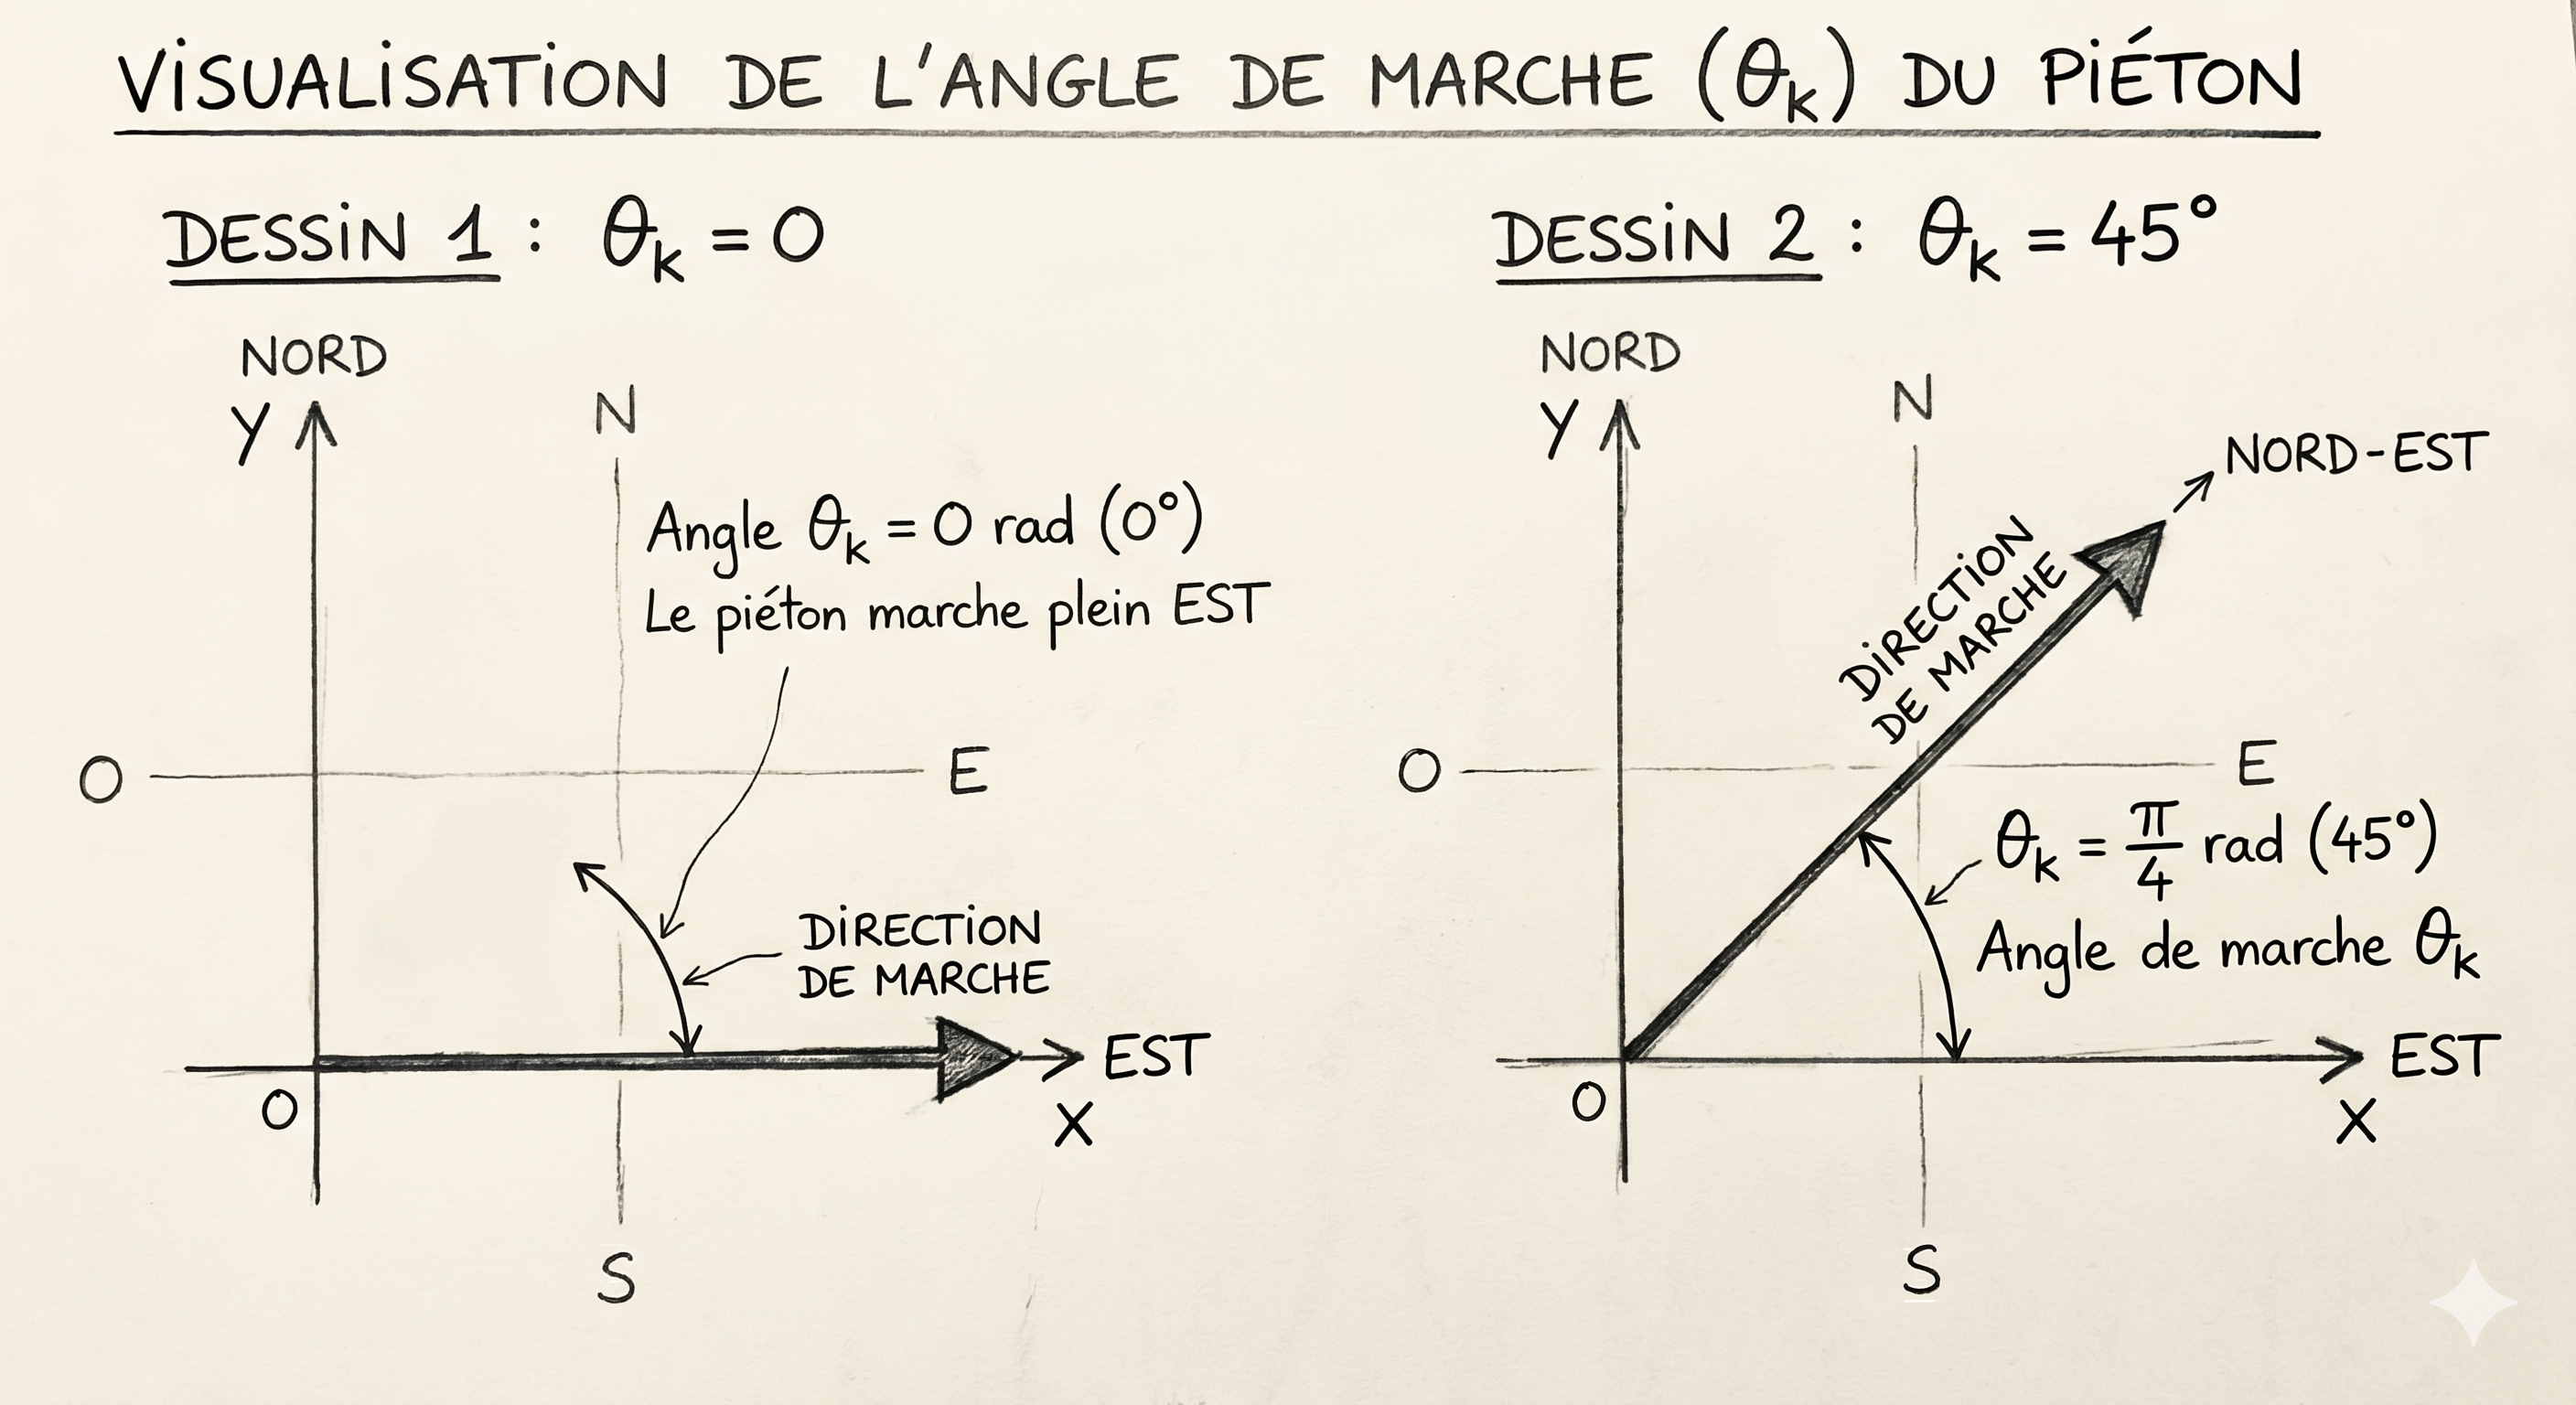
\includegraphics[width=0.5\textwidth]{images/model_boussole.png}
    \caption{Modèle de la boussole et repère Est-Nord}
    \label{fig:model_boussole}
\end{figure}

Le système est piloté par le vecteur de commande $U_k$ :
\begin{equation}
 U_k = \begin{bmatrix} v_k \\ \omega_k \end{bmatrix} 
\end{equation}
Où $v_k$ est la vitesse scalaire du piéton et $\omega_k$ la vitesse angulaire. 
Dans notre montage matériel, nous avons observé expérimentalement que l'accéléromètre mesurait systématiquement environ $1G$ (la gravité terrestre) sur l'axe X, tandis que les axes Y et Z restaient proches de $0G$. On en deduit que la carte Raspberry Pi était fixée de sorte que son axe X pointait verticalement vers le ciel. Donc la rotation du piéton sur lui-même correspond physiquement à une rotation autour de cet axe vertical, qui est lue directement par \textit{Gyro\_X} (IMU).

\begin{figure}[htbp]
    \centering
    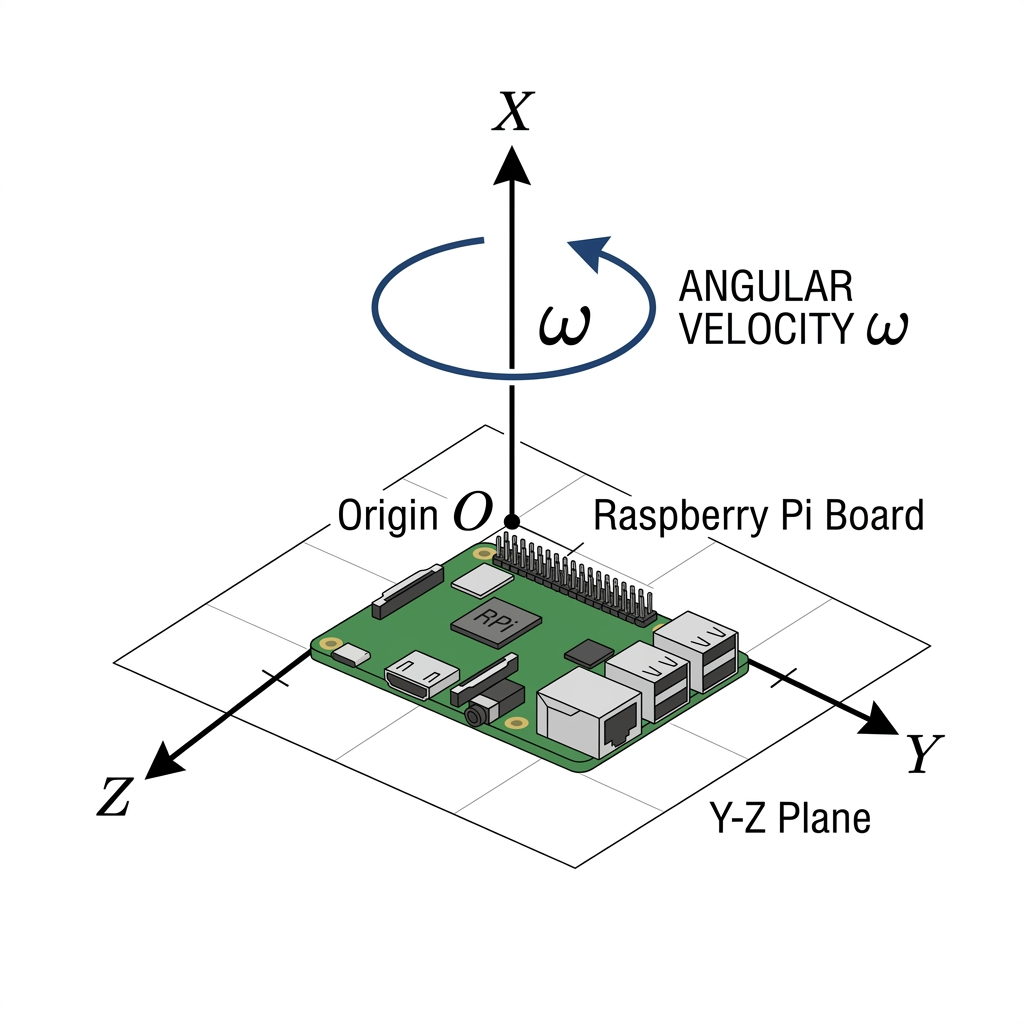
\includegraphics[width=0.5\textwidth]{images/diagramme_imu_axe_x.png}
    \caption{Montage matériel de l'IMU : l'axe X pointe vers le haut}
    \label{fig:diagramme_imu_axe_x}
\end{figure}

\subsubsection{Étape de Prédiction (Propagation)}
L'évolution de la position du piéton n'est pas linéaire à cause des fonctions trigonométriques. Le modèle non-linéaire $f$ se traduit par les équations de mécanique classique :
\begin{equation}
 \begin{bmatrix} x_k \\ y_k \\ \theta_k \end{bmatrix} = \begin{bmatrix} x_{k-1} + v_k \cdot \cos(\theta_{k-1}) \cdot \Delta t \\ y_{k-1} + v_k \cdot \sin(\theta_{k-1}) \cdot \Delta t \\ \theta_{k-1} + \omega_k \cdot \Delta t \end{bmatrix} 
\end{equation}

\begin{figure}[htbp]
    \centering
    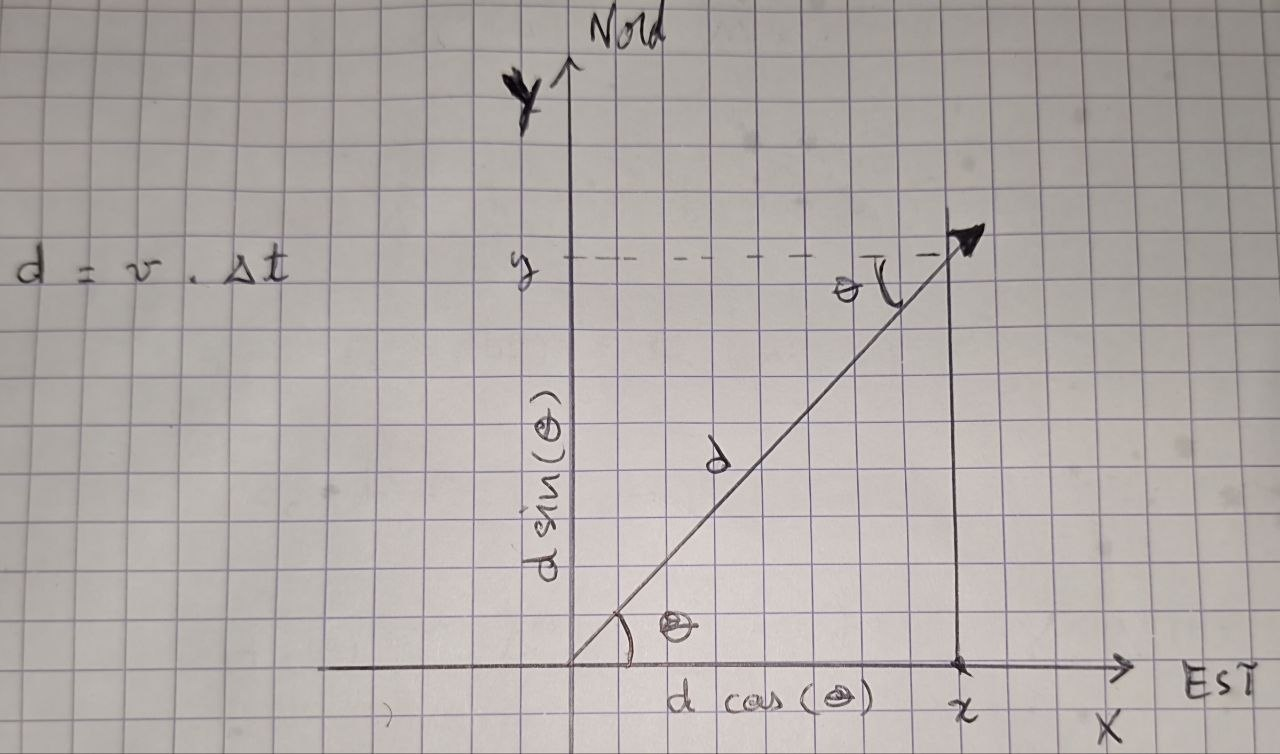
\includegraphics[width=0.5\textwidth]{images/trigo_cinematique.jpg}
    \caption{Projection trigonométrique du déplacement $v \cdot \Delta t$ sur les axes Est ($X$) et Nord ($Y$)}
    \label{fig:trigo_cinematique}
\end{figure}

Pour appliquer le filtre de Kalman, nous devons linéariser cette fonction en calculant sa Jacobienne $F_k$ :
\begin{equation}
 F_k = \frac{\partial f}{\partial X} = \begin{bmatrix} 1 & 0 & -v_k \cdot \sin(\theta_{k-1}) \cdot \Delta t \\ 0 & 1 & v_k \cdot \cos(\theta_{k-1}) \cdot \Delta t \\ 0 & 0 & 1 \end{bmatrix} 
\end{equation}

\textbf{Matrice de Bruit de Processus ($Q$)} \\
La matrice de covariance $Q$ représente l'incertitude de notre prédiction. Issue du modèle \textbf{CWNA} (\textit{Continuous White Noise Acceleration}, réf. CM6), elle se modélise par :
\begin{equation}
 Q = \begin{bmatrix} \frac{\sigma_a^2 \cdot \Delta t^4}{4} & 0 & 0 \\ 0 & \frac{\sigma_a^2 \cdot \Delta t^4}{4} & 0 \\ 0 & 0 & \sigma_\omega^2 \cdot \Delta t^2 \end{bmatrix} 
\end{equation}
Ici, $\sigma_a$ est recalculé dynamiquement à chaque itération via la variance de l'accélération horizontale de l'IMU, permettant au filtre de s'adapter à la force réelle du pas de l'utilisateur.
La prédiction de la covariance devient alors : $P_{k|k-1} = F_k P_{k-1|k-1} F_k^T + Q$.

\subsubsection{Étape de Correction (Mise à jour GPS)}
Nous mesurons uniquement la position $(x, y)$ grâce au GPS. La matrice d'observation $H$ est donc linéaire :
\begin{equation}
 H = \begin{bmatrix} 1 & 0 & 0 \\ 0 & 1 & 0 \end{bmatrix} 
\end{equation}

La matrice $R$ représente l'imprécision du GPS, obtenue expérimentalement lors de nos tests :
\begin{equation}
 R = \begin{bmatrix} 1.20 & 0 \\ 0 & 0.07 \end{bmatrix} 
\end{equation}

\textbf{Filtre Anti-Outliers (Distance de Mahalanobis)} \\
Afin de rejeter les mesures GPS aberrantes (phénomène de \textit{multipath} ou pertes de signal temporaires), nous avons implémenté une technique de \textit{gating} probabiliste basée sur la distance de Mahalanobis. Avant d'accepter une mesure GPS, nous calculons l'innovation $\tilde{y} = Z_k - H \hat{X}_{k|k-1}$ et sa covariance $S = H P_{k|k-1} H^T + R$.
Nous évaluons ensuite la distance de Mahalanobis au carré : $d^2 = \tilde{y}^T S^{-1} \tilde{y}$. 

Statistiquement, les résidus normalisés d'un filtre de Kalman optimal suivent une loi du $\chi^2$ (Khi-deux). Pour notre système d'observation 2D (X et Y), nous avons 2 degrés de liberté.
Pour rejeter les données aberrantes avec un intervalle de confiance de 99\%, le seuil théorique tabulé est de $9.21$ (\textit{Réf : Tables statistiques du $\chi^2$ / Théorie de l'estimation et du filtrage optimal}). 
Ainsi, si $d^2 > 9.21$, la mesure GPS est considérée comme une anomalie et est purement ignorée, laissant le modèle inertiel prendre le relais pour garantir la fluidité de la trajectoire.

Si la mesure est valide, nous calculons le gain de Kalman $K$ et corrigeons l'état :
\begin{align}
   K &= P_{k|k-1} H^T S^{-1} \\
   \hat{X}_{k|k} &= \hat{X}_{k|k-1} + K \tilde{y} \\
   P_{k|k} &= (I - K H) P_{k|k-1}
\end{align}

\subsection{Critique et Limites du Modèle}

Bien que robuste face aux interférences magnétiques et au bruit d'accélération, notre modèle EKF cinématique repose sur plusieurs hypothèses:

\begin{enumerate}
    \item \textbf{Dépendance à la vitesse déduite du GPS} : Actuellement, la vitesse scalaire $v_k$ est calculée à partir de la différence de position entre deux points GPS successifs. Une amélioration  consisterait à récupérer et utiliser directement la vitesse \textit{Doppler} native fournie par la puce GPS (via les trames NMEA originelles). Cette vitesse matérielle est nettement plus instantanée et fiable que la dérivation spatiale. De plus, si le signal GPS est totalement perdu (ex: tunnel prolongé), notre vitesse calculée tombe à zéro, empêchant toute vraie navigation (mais cela peut se resoudre en integrant temporairement l'acceleration).
    \item \textbf{Dérive résiduelle du Gyroscope (Drift)} : En l'absence d'un cap absolu (le magnétomètre ayant été écarté du modèle en raison des perturbations environnementales), l'intégration numérique de la vitesse angulaire $\omega_k$ finira inévitablement par dériver au bout de plusieurs dizaines de minutes de marche, malgré notre calibration statique du biais initial.
    \item \textbf{Hypothèse de mouvement rectiligne aligné} : Le modèle cinématique suppose que le piéton avance en permanence de manière parfaitement alignée avec l'axe de visée de la carte (cap $\theta$). Cette restriction rend le modèle incapable d'estimer correctement la trajectoire lors de mouvements tels que les pas chassés ou les marches en reculant ... (personne ne fait ça normalement)
\end{enumerate}

Nous avons pas pu exploiter le magnetomètre comme il se devait il resoudrait bon nombre de nos problèmes.

\section{Partie 2 : Fonctionnalité supplémentaire}
\subsection{L'idée initiale}
Suite à une première concertation au sein du groupe, nous avons décidé de coder une fonctionnalité qui nous permettrait de localiser des photos prises sur une carte. Après consultation avec les professeurs, nous avons ajouter à cette idée une fonctionnalité de résolution de parcours. Cette dernière, nous permet de créer une sorte de GeoGuessr. 

\subsection{Mode d'emploi}
\subsubsection{Construction du parcours}
La première étape est de construire.final(aaaaaaaaaaaaaaaaaaaaaaaaaaaaaaaa)

\subsubsection{Résolution du parcours}


\end{document}